%!TEX options = -shell-escape

\documentclass[glossy]{beamer}
\usepackage[utf8]{inputenc} % Unicode support (Umlauts etc.)
\usepackage{graphicx} % Add pictures to your document
\usepackage{hyperref} % Add a link to your document
\usepackage{minted}
\usepackage{tikz}
\usepackage{lmodern}
\usepackage[T1]{fontenc}

\useoutertheme{wuerzburg}
\useinnertheme[realshadow,corners=2pt,padding=2pt]{chamfered}
\usecolortheme{shark}

\setbeamertemplate{navigation symbols}{}

\usetikzlibrary{tikzmark, arrows, decorations, decorations.pathreplacing}
\newminted{cpp}{autogobble, fontsize=\tiny, escapeinside=@@}
\newmintinline{cpp}{}
\newmintinline{java}{}
\newmintinline{js}{}
\usemintedstyle{vs}

\tikzset{every picture/.style={font issue=\scriptsize},
         font issue/.style={execute at begin picture={#1\selectfont}}
        }


\title{C++ Boot Camp 1/2}
\author{Jesse Talavera-Greenberg}
\date{\today}

% Concepts to cover:
% const-correctness
% Value semantics
% OOP
% Exception safety
% C++ vs C
% Concepts
\begin{document}

\newcommand{\cppref}[2]{\href{http://en.cppreference.com/w/cpp/#1}{\underline{#2}}}

\begin{frame}
\maketitle
\end{frame}

\begin{frame}
\frametitle{This Week}
  \begin{itemize}
    \item No need to download anything this week
    \item Go to \href{www.cppreference.com}{www.cppreference.com} to follow code
    \item This is your C++ Bible this semester
    \item Online compiler
  \end{itemize}
\end{frame}

\begin{frame}
\frametitle{Disclaimer}
    \begin{itemize}
        \item I am not the grader for this course
        \begin{itemize}
            \item Undergrads can't grade assignments
        \end{itemize}
        \item The boot camp is always part of the course, but I volunteered to lead it this year.
        \item Any opinions expressed are my own and are not necessarily condoned by McKenna.
        \item I don't know very much about DirectX.
    \end{itemize}
\end{frame}

\begin{frame}
  \frametitle{Today}
  \begin{itemize}
    \item Core language features
    \item Memory management
    \item Gotchas
    \item How to do common things
  \end{itemize}
\end{frame}

\begin{frame}
  \frametitle{Distinct Points}
  \begin{itemize}
    \item Balance high-level language constructs and low-level resource management
    \item Huge-ass language
    \item Designed for C compatibility
    \item Accumulated lots of cruft over the years
  \end{itemize}
\end{frame}

\begin{frame}
  \frametitle{C vs. C++}
  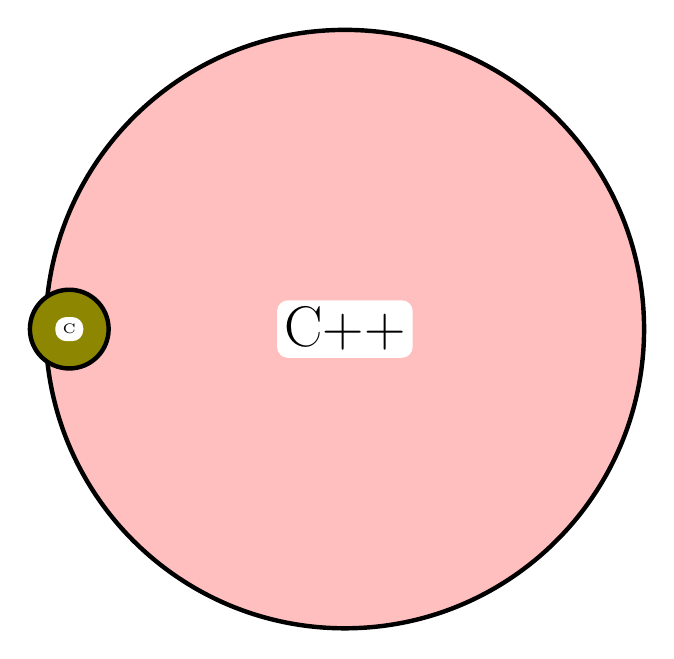
\begin{tikzpicture}
    \draw [fill=pink, ultra thick] (16,8) circle (3.8cm) node [align=center, anchor=center, fill=white, rounded corners] {\huge{C++}};
    \draw [fill=olive, ultra thick] (12.5,8) circle (.5cm) node [align=center, anchor=center, fill=white, rounded corners] {\tiny{C}};
  \end{tikzpicture}
\end{frame}

\begin{frame}[fragile=singleslide]
  \frametitle{The Basics}
  \begin{cppcode}
#include <iostream>@\tikzmark{basic_include}@

// Comments
/* Block comments */
using std::cout; @\tikzmark{basic_using_a}@
using std::endl; @\tikzmark{basic_using_b}@

const int SOME_CONSTANT = 5;

// Main entry point of a C++ program
int @\cppref{language/main_function}{main}@(int argc@\tikzmark{basic_argc}@, char** argv@\tikzmark{basic_argv}@) {
  // main() args are optional

  for (int i = 0; i < argc; ++i) {
    cout << "Arg #" << i << ": " << argv[i] << endl;@\tikzmark{basic_print}@
  }

  cout << "You gave ";
  switch (argc) {@\tikzmark{basic_switch}@
    case 0:
      cout << "exactly ";
    case SOME_CONSTANT:
      cout << SOME_CONSTANT;
      break;
    default:
      cout << "some number of"
  }
  cout << " arguments." << endl;

  return 0;@\tikzmark{basic_return}@
}
  \end{cppcode}

  
\begin{tikzpicture}[remember picture, ->, >=stealth, overlay, red, ultra thick, align=left]
    \draw (4.5cm, 26em) node [anchor=west] {\shortstack{Include libraries, functions, etc.}} -> ([shift={(.25em,.25em)}]pic cs:basic_include);
    \draw (7cm, 24em) node [anchor=west] {\shortstack{\# of command-line arguments}} -> ([shift={(.25em,.25em)}]pic cs:basic_argc);
    \draw (7cm, 21em) node [anchor=west] {\shortstack{actual arguments as\\a string array}} -> ([shift={(.25em,.25em)}]pic cs:basic_argv);
    \draw[decorate, decoration={brace}, -] ({pic cs:basic_using_a} |- {pic cs:basic_using_b}) +(0,1.5em) -- node [right, inner sep=1em] {Pulls into namespace\\(avoid long-ass prefixes)} ({pic cs:basic_using_a} |- {pic cs:basic_using_b});
    \draw (7cm, 15em) node [anchor=west] {\shortstack{Formatted printout}} -> ([shift={(.25em,.25em)}]pic cs:basic_print);
    \draw (5cm, 3em) node [anchor=west] {\shortstack{Return code (absence in main implies 0)}} -> ([shift={(.25em,.25em)}]pic cs:basic_return);
    \draw (4cm, 12em) node [anchor=west] {\shortstack{Strings not allowed\\in switch statements}} -> ([shift={(.25em,.25em)}]pic cs:basic_switch);
  \end{tikzpicture}
\end{frame}

\begin{frame}[fragile=singleslide]
  \frametitle{Fundamental Types}
  \begin{columns}[t]
    \begin{column}{6cm}
      \begin{itemize}
        \item Integer sizes \textbf{can vary} by platform, compiler, and OS
        \item No \javainline|byte| (use \cppinline|uint8_t|)
        \item \javainline|boolean| $\rightarrow$ \cppinline|bool|
        \item Numbers implicitly convert to \cppinline|bool| (0 $\rightarrow$ \javainline|false|, anything else $\rightarrow$ \javainline|true|)
        \item Use \cppinline|nullptr| for null pointers, not \javainline|null| or \cppinline|NULL|
        \item \cppinline|float| and \cppinline|double| are the same as in Java (\cppinline|long double| exists, too)
      \end{itemize}
    \end{column}

    \begin{column}{6cm}
      \begin{itemize}
        \item \cppinline|signed| and \cppinline|unsigned| integers
        \begin{itemize}
          \item \cppinline|signed| integers are the same
          \item \cppinline|unsigned| go twice as high, but no negatives
        \end{itemize}
        \item For specific sizes, \cppinline|#include <cstdint>| and use \jsinline{/std::u?int(8|16|32|64)_t/}
        \item There is \textbf{no} root object class
      \end{itemize}
    \end{column}
  \end{columns}
\end{frame}

\begin{frame}[fragile=singleslide]
  \frametitle{Exceptions}
  \begin{cppcode}
#include <exception> @\tikzmark{except_header}@

using std::exception;

int couldThrow(int x) {@\tikzmark{except_nocheck}@
  if (x % 2 == 0) throw exception("No new statement (more info later)");
  return x;
}

int willNotThrow(int x) noexcept {@\tikzmark{except_noexcept}@
  return x * x;
}

int functionThrow(int x) try {@\tikzmark{except_function}@
  return couldThrow(x);
}
catch (exception e) {
  return x + 1;  // Can still access parameters
}

int main(int argc) {
  int a = willNotThrow(argc);
  try {  
    couldThrow(functionThrow(a));
  }
  catch (exception e)@\tikzmark{except_type}@ {
    std::cout << e.what();
  }
  catch (...) {@\tikzmark{except_swallow}@
    std::cout << "What the fuck?";
  }@\tikzmark{except_nofinally}@
}
  \end{cppcode}

  
\begin{tikzpicture}[remember picture, ->, >=stealth, overlay, red, ultra thick, align=left]
    \draw (4cm, 27em) node [anchor=west] {\shortstack{Contains exception handling\\classes and functions}} -> ([shift={(.25em,.25em)}]pic cs:except_header);
    \draw (5cm, 21em) node [anchor=west] {\shortstack{Will not throw an exception\\(program terminates if it does)}} -> ([shift={(.25em,.25em)}]pic cs:except_noexcept);
    \draw (6cm, 18em) node [anchor=west] {\shortstack{Not often used, but may come in handy}} -> ([shift={(.25em,.25em)}]pic cs:except_function);
    \draw (5cm, 9em) node [anchor=west] {\shortstack{Base exception type\\(any type can be thrown, but use these)}} -> ([shift={(.25em,.25em)}]pic cs:except_type);
    \draw (6cm, 4em) node [anchor=west] {\shortstack{No finally statement\\(use destructors instead)}} -> ([shift={(.25em,.25em)}]pic cs:except_nofinally);
  \end{tikzpicture}
\end{frame}

\begin{frame}[fragile=singleslide]
  \frametitle{Type Aliases}
  \begin{cppcode}
#include <array>
#include <cstdint>
#include <iostream>
#include <typeinfo>@\tikzmark{typedef_typeinfo}@

using byte = std::uint8_t;@\tikzmark{typedef_using_a}@

template<class T>
using Array10 = std::array<T, 10>;@\tikzmark{typedef_using_b}@

// Traditional syntax uses "typedef" keyword:@\tikzmark{typedef_prefer}@
//    typedef existing_type new_name;
using std::cout;
using std::endl; 

int main() { 
  std::uint8_t a = 5;@\tikzmark{typedef_okay_a}@
  byte b = a;@\tikzmark{typedef_okay_b}@

  cout << typeid(std::uint8_t).name() << ' ' << typeid(byte).name() << endl;@\tikzmark{typedef_same_a}@

  Array10<byte> c;

  cout << typeid(std::array<byte, 10>).name() << ' ' << typeid(c).name() << endl;@\tikzmark{typedef_same_b}@

  // Many standard types are typedefs (but this is hidden from you)
}
  \end{cppcode}

  
\begin{tikzpicture}[remember picture, ->, >=stealth, overlay, red, ultra thick, align=left]
    \draw (4cm, 22em) node [anchor=west] {\shortstack{Needed for the\\typeid operator}} -> ([shift={(.25em,.25em)}]pic cs:typedef_typeinfo);
    \draw (3cm, 10.5em) node [anchor=west] {\shortstack{Difference is compile-time only}} -> ([shift={(.25em,.25em)}]pic cs:typedef_okay_a);
    \draw (3cm, 10.5em) -> ([shift={(.25em,.25em)}]pic cs:typedef_okay_b);
    \draw (6cm, 16em) node [anchor=west] {\shortstack{Prefer using, but recognize typedef}} -> ([shift={(.25em,.25em)}]pic cs:typedef_prefer);
    \draw (10cm, 11em) node [anchor=south] {\shortstack{Both strings are the same\\(but implementation-defined)}} -> ([shift={(.25em,.25em)}]pic cs:typedef_same_a);
    \draw (10cm, 11em) -> ([shift={(.25em,.25em)}]pic cs:typedef_same_b);
    \draw (6cm, 19em) node [anchor=west] {\shortstack{Another name for\\the same type}} -> ([shift={(.25em,.25em)}]pic cs:typedef_using_a);
    \draw (6cm, 19em) -> ([shift={(.25em,.25em)}]pic cs:typedef_using_b);
  \end{tikzpicture}
\end{frame}

\begin{frame}[fragile=singleslide]
  \frametitle{Memory Model and Lifetime}
  \begin{columns}
    \begin{column}{6cm}
      \begin{itemize}
        \item \textbf{static:} Exists for program's entire duration (on stack or in program data)\tikzmark{memory_static_a}
        \item \textbf{automatic:} Disappears when out of scope (on stack)\tikzmark{memory_auto_a}
        \item \textbf{dynamic:} Created and destroyed at will (on heap)\tikzmark{memory_dynamic_a}
        \begin{itemize}
          \item Remember to clean up (one \cppinline{delete} for every \cppinline{new})
        \end{itemize}
      \end{itemize}
    \end{column}

    \begin{column}{6cm}
      \begin{cppcode}
#include <string>

using std::string;

@\tikzmark{memory_static_b}@string a = "I'll always exist";

void scope() {
  @\tikzmark{memory_auto_b}@string b = "I'll die at the end of the block";
  @\tikzmark{memory_dynamic_b}@string* c = new string("I'll die when you kill me");

  delete c; // c is deleted
  // b is deleted
}

int main() {
  for (int i = 0; i < 100000; ++i) {
    @\tikzmark{memory_dynamic_c}@string* d = new string("Oops");
    // d is not deleted (all 100000 instances of it)
  }

  // a is deleted
}
      \end{cppcode}
    \end{column}
  \end{columns}

  
\begin{tikzpicture}[remember picture, ->, >=stealth, overlay, red, ultra thick, align=left]
    \draw (pic cs:memory_static_a) -> ([shift={(0em,.25em)}]pic cs:memory_static_b);
    \draw (pic cs:memory_auto_a) -> ([shift={(0em,.25em)}]pic cs:memory_auto_b);
    \draw (pic cs:memory_dynamic_a) -> ([shift={(0em,.25em)}]pic cs:memory_dynamic_b);
    \draw (pic cs:memory_dynamic_a) -> ([shift={(0em,.25em)}]pic cs:memory_dynamic_c);
  \end{tikzpicture}
\end{frame}

\begin{frame}[fragile=singleslide]
  \frametitle{Memory Model and Lifetime (cont'd)}
  \begin{columns}
    \begin{column}{6cm}
      \begin{itemize}
        \item Stack allocation is fast, but size must be known at compile time
        \item Heap allocation is flexible, but slow
        \item Details vary by compiler, OS, and hardware
        \item \textbf{All objects of a given type are the same size.}
      \end{itemize}
    \end{column}

    \begin{column}{6cm}
      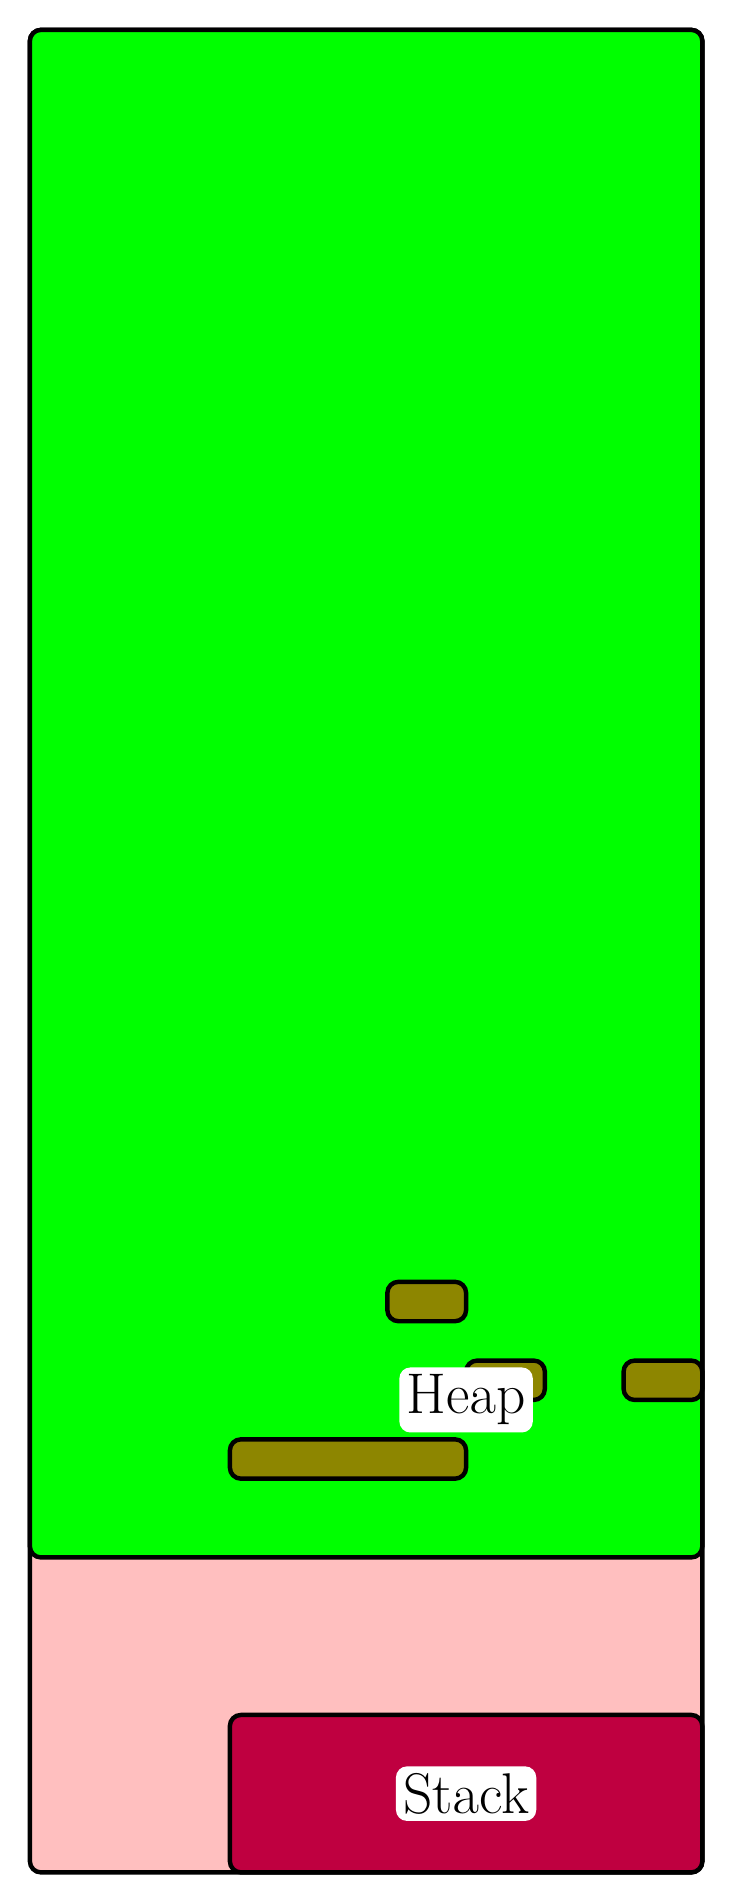
\begin{tikzpicture}
        \draw [fill=pink, ultra thick, rounded corners] (current page.north west) rectangle (6cm, 2cm);
        \draw [fill=purple, ultra thick, rounded corners] (0cm, 2cm) rectangle (6cm, 4cm) node [align=center, anchor=center, fill=white] at (3cm, 3cm) {\huge{Stack}};
        \draw [fill=green, ultra thick, rounded corners] (current page.north west) rectangle (6cm, 6cm);
        \draw [fill=olive, ultra thick, rounded corners] (2cm, 9cm) rectangle +(1cm, 0.5cm) (3cm, 8cm) rectangle +(1cm, 0.5cm) (5cm, 8cm) rectangle +(1cm, 0.5cm) (0, 7cm) rectangle +(3cm, 0.5cm);
        \draw node [align=center, anchor=center, fill=white, rounded corners] at (3cm, 8cm) {\huge{Heap}};
      \end{tikzpicture}
    \end{column}
  \end{columns}

  \begin{tikzpicture}[remember picture, ->, >=stealth, overlay, red, ultra thick, align=left]
    \draw (4cm, 22em) node [anchor=east] {\shortstack{Find enough space (expensive)}} -> (6.25cm, 5.25cm);
    \draw (4cm, 3em) node [anchor=east] {\shortstack{Increment an address (cheap)}} -> (6.25cm, 1cm);
  \end{tikzpicture}
\end{frame}

\begin{frame}[fragile=singleslide]
  \frametitle{Pointers Vs. References}

  \begin{itemize}
    \item Access lots of data without copying it
    \item Left dangling (\textbf{invalid}) if the referenced object is deallocated
    \begin{itemize}
      \item No way to check for this
      \item Will likely cause a crash if you try to use it
    \end{itemize}
    \item Polymorphism okay
    \item Both compile to similar machine code
    \item Multiple pointers/references can refer to one object
  \end{itemize}

  \begin{columns}
    \begin{column}{6cm}
      \textbf{Pointers:}
      \begin{itemize}
        \item More prone to becoming invalid
        \item Can represent absence of data (\cppinline{nullptr})
        \item Syntax to use and declare
        \item Address can be reassigned
      \end{itemize}
    \end{column}

    \begin{column}{6cm}
      \textbf{References:}
      \begin{itemize}
        \item Must initialize properly
        \item Always points to \textbf{one} address
        \item No syntax to use, only to declare
        \item Easier to deal with objects that shouldn't change
      \end{itemize}
    \end{column}
  \end{columns}
\end{frame}

\begin{frame}[fragile=singleslide]
  \frametitle{Pointers and References}
  \begin{columns}[t]
    \begin{column}{6cm}
      \textbf{Pointers:}
      \begin{cppcode}
#include <iostream>

using std::cout;
using std::endl;

struct Base {
  int enormous[1024];
};

struct Derived : public Base {
  float huge[1024];
};

int main() {
  Base base;
  Derived derived;
  
  Base* a = &base;
  Base* b = &derived; // Polymorphism
  Base* c; // Uninitialized (value undefined)
  c = nullptr;
  c = &derived; // Changed pointer
  
  const Base* d = a; // mutable pointer, const data
  Base const* e = a; // const pointer, mutable data
  const Base* const f = a; // pointer and data const
  
  int* ptr = a->enormous; // Pointer arithmetic
  cout << *ptr << *(ptr + 1) << (*ptr) + 1 << endl;
}
      \end{cppcode}
    \end{column}

    \begin{column}{6cm}
      \textbf{References:}
      \begin{cppcode}
#include <iostream>

using std::cout;
using std::endl;

struct Base {
  int enormous[1024];
};

struct Derived : public Base {
  float huge[1024];
};

int main() {
  Base base;
  Derived derived;
  
  Base& a = base;
  Base& b = derived; // Polymorphism
  // References must be initialized
  // And to a valid object, too
  a = derived; // Changed pointee (the object)
  
  const Base& d = a; // const data
  // References never change (they always point
  // to one address)

  cout << a.enormous[0] << a.enormous[1] << endl;
}
      \end{cppcode}
    \end{column}
  \end{columns}
\end{frame}

\begin{frame}[fragile=singleslide]
  \frametitle{Undefined Behavior}
  \begin{columns}
    \begin{column}{6cm}
      \begin{itemize}
        \item Java fully defines everything
        \item C++ leaves certain edge cases up to the compiler
        \item Many, many ways to invoke
        \item \textbf{Do not rely on UB}
        \begin{itemize}
          \item Best case scenario: Crash
          \item Worst case scenario: No crash
        \end{itemize}
      \end{itemize}
    \end{column}

    \begin{column}{6cm}
      \begin{cppcode}
#include <string>
#include <limits>

using std::string;

int something(int param) { 
  if (param > 0) return param; 
  // No return down here; now what? 
} 

string& returnsALocal() { 
  string reference = "Why are you doing this"; 
  return reference; // Uh-oh 
} 

int main() { 
  int a = std::numeric_limits<int>::max(); 
  a++; // Oops 

  int* pointer; // What's inside?  Beats me.
  int number = *pointer;

  int[10] array; 
  number = array[12]; // WTF 
}
      \end{cppcode}
    \end{column}
  \end{columns}
\end{frame}

\begin{frame}[fragile=singleslide]
  \frametitle{Namespaces}
  \begin{cppcode}
#include <iostream>
#include <string>
#include <array>
#include <utility>

using namespace std;@\tikzmark{namespace_std}@

namespace sbcs {@\tikzmark{namespace_nest_a}@
  namespace cse380 {@\tikzmark{namespace_nest_b}@
    struct Game {
      string name;
      string teamName;
      array<string, 3> members;
    };
  }

  namespace cse381 {@\tikzmark{namespace_nest_c}@
    using Team = pair<string, string>;
  }
}

int main() {
  sbcs::cse380::Game game;@\tikzmark{namespace_qualified}@
  using sbcs::cse381::Team;@\tikzmark{namespace_using}@

  Team team("Jesse", "Karl");
}
  \end{cppcode}

  
\begin{tikzpicture}[remember picture, ->, >=stealth, overlay, red, ultra thick, align=left]
    \draw (6cm, 22em) node [anchor=west] {\shortstack{Don't do this (or java.util.*)}} -> ([shift={(0em,.25em)}]pic cs:namespace_std);
    \draw (5cm, 19em) node [anchor=west] {\shortstack{Nest them as much as you'd like}} -> ([shift={(0em,.25em)}]pic cs:namespace_nest_a);
    \draw (5cm, 19em) -> ([shift={(0em,.25em)}]pic cs:namespace_nest_b);
    \draw (5cm, 19em) -> ([shift={(0em,.25em)}]pic cs:namespace_nest_c);
    \draw (5cm, 8em) node [anchor=west] {\shortstack{Fully-qualified name}} -> ([shift={(0em,.25em)}]pic cs:namespace_qualified);
    \draw (6cm, 4em) node [anchor=west] {\shortstack{Or bring it into the\\current namespace}} -> ([shift={(0em,.25em)}]pic cs:namespace_using);
  \end{tikzpicture}
\end{frame}

\begin{frame}[fragile=singleslide]
  \frametitle{The Preprocessor}
  \begin{cppcode}
#include <iostream>@\tikzmark{cpp_include}@

#define DEBUG@\tikzmark{cpp_define}@

// #define WINDOWS@\tikzmark{cpp_windows}@
// #define MAC@\tikzmark{cpp_mac}@

using std::cout; 
using std::endl; 

int main() { 
  #ifdef DEBUG 
  cout << "Logging! Or sanity checking!" << endl;
  #endif 

  #ifdef WINDOWS
  cout << "Use DirectX!" << endl; 
  #else 
  cout << "Use OpenGL!" << endl; 
  #endif

  #ifndef LINUX@\tikzmark{cpp_linux}@
  cout << "Why do you hate penguins?" << endl;
  #endif

  #ifdef MAC 
    #error "Jesse doesn't like Apple"@\tikzmark{cpp_error}@
  #endif
}
  \end{cppcode}

  
\begin{tikzpicture}[remember picture, ->, >=stealth, overlay, red, ultra thick, align=left]
    \draw (3cm, 25em) node [anchor=west] {\shortstack{Convention: <> for third-party or\\standard library, "" for your code}} -> ([shift={(0em,.25em)}]pic cs:cpp_include);
    \draw (4cm, 21em) node [anchor=west] {\shortstack{Conditional compilation (you can also add\\\#defines through your build process)}} -> ([shift={(0em,.25em)}]pic cs:cpp_define);
    \draw (3cm, 18em) node [anchor=west] {\shortstack{Uncomment these}} -> ([shift={(0em,.25em)}]pic cs:cpp_windows);
    \draw (3cm, 18em) -> ([shift={(0em,.25em)}]pic cs:cpp_mac);
    \draw (4cm, 9em) node [anchor=west] {\shortstack{Contents ignored (not compiled) if on Linux}} -> ([shift={(0em,.25em)}]pic cs:cpp_linux);
    \draw (5cm, 3em) node [anchor=west] {\shortstack{Intentional compiler error}} -> ([shift={(0em,.25em)}]pic cs:cpp_error);
  \end{tikzpicture}
\end{frame}

\begin{frame}[fragile=singleslide]
  \frametitle{enums}
  \begin{cppcode}
#include <iostream> 

using std::cout; 
using std::endl; 

enum class Direction { 
  North, 
  South, 
  East,
  West, // Trailing comma is okay 
}; 

// NOT OBJECTS; just ints with some compile-time meaning 
enum class Speakers { 
  Mute = 0, // Assigning values is okay 
  Mono = 1, 
  Stereo = 2, 
  Surround = 4 
}; 

int main() { 
  Direction dir = Direction::North;
  Speakers audio = Speakers::Stereo;
  audio = Speakers(4); // Make sure int is a valid Speakers value!
  cout << int(audio) << endl;
  // int <-> enum class conversions must be explicit
}
  \end{cppcode}
\end{frame}

};


}
  \end{cppcode}

\end{frame}

\begin{frame}[fragile=singleslide]
  \frametitle{new/delete}
  \begin{cppcode}
#include <string>

using std::string;

void wasteMemory() {
  string stack_allocated = "I disappear when I go out of scope";
  string* wasted = new string("I only disappear when explicitly deallocated");

  string* cleaned = new string("I'm about to get cleaned up properly");

  delete cleaned;
}

int main() {
  for (int i = 0; i < 10000; i++) {
    wasteMemory();
  }

  // stack_allocated disappeared when wasteMemory() returned
  // All instances of wasted are still in memory
  // cleaned disappeared when "delete cleaned;" was called
  // See: Scope vs. Lifetime
}
  \end{cppcode}
\end{frame}

\begin{frame}[fragile=singleslide]
  \begin{cppcode}


  \end{cppcode}
\end{frame}

\begin{frame}[fragile=singleslide]
  \frametitle{Declaring Classes}
  \begin{cppcode}
// public/protected/private semantics same as in Java
// no specifier == private in classes, public in structs

class ItHoldsThings {
  public: 
    int cantBeOverridden(int a, int b) {
      // Technically you can, but things get weird
      return this->_integer + b;
    }

    virtual float canBeOverridden(const double d) {
      // virtual == overrideable
      return d * 2;
    }

    virtual void abstractMethod() = 0;

  protected:
    float _number;

  private:
    int _integer;
}; // Don't forget the semicolon
// When a class is constructed, ALL of its members are too
  \end{cppcode}
\end{frame}

\begin{frame}[fragile=singleslide]
  \frametitle{Constructors}
  \begin{cppcode}
#include <string>

using std::string; 

class StringWrapper { 
  public: 
    StringWrapper() { /* other code here */ } // _str == ""
    // Default constructor can be auto-generated with some caveats (see the wiki)

    StringWrapper(const string& value) : _str(value) {} // _str == value
    // Copy constructor can be auto-generated (but see wiki)
    // Base class constructors are called like this, too

  private:
    string _str;
    // All members are initialized on construction, whether you like it or not
};

int main() { 
  StringWrapper a;
  StringWrapper b("There will be a copy of me in c");
  StringWrapper c(b);
}
  \end{cppcode}
\end{frame}

\begin{frame}[fragile=singleslide]
  \frametitle{Destructors}
  \begin{cppcode}
// Using constructors to allocate resources and destructors to clean them up is 
// called Resource Acquisition Is Initialization (RAII). Only needed for low-level 
// resources; high-level classes like std::iostream do RAII themselves. 

#include <cstdlib> 

using std::malloc;
using std::free;

class LotsOfResources {
  public:
    LotsOfResources() {
      _floats = new float[64];
      _buffer = malloc(64);
    }

    ~LotsOfResources() {
      // Called when this object's lifetime ends delete[] _floats;
      // Remember the [] when deleting a raw array free(_buffer);
    }

  private:
    float* _floats;
    void* _buffer;
};

int main() {
  LotsOfResources* resources = new LotsOfResources;
  delete resources; // No memory leaks!
}
  \end{cppcode}
\end{frame}

\begin{frame}[fragile=singleslide]
  \frametitle{new/delete}
  \begin{cppcode}
  \end{cppcode}
\end{frame}

\begin{frame}[fragile=singleslide]
  \frametitle{Abstract classes and inheritance}
  \begin{cppcode}
#include <exception> 
#include <iostream> 

// There are no interfaces; use abstract classes without any concrete methods 
struct ProgramCrasher { 
  virtual void crash() = 0; // "= 0" means the method is abstract 
  // virtual == method can be overridden 
  // only one abstract method needed to define a class as abstract
}; 

struct IPastryChef { 
  virtual void bake() = 0; 
};

struct SegfaultCrasher : public ProgramCrasher {
  // Actually several types of inheritance; it's complicated, just use public

  void crash() override {
    int* a;
    int b = *a;
  }
};
// Multiple inheritance; don't do it if more than one parent class is not an interface

struct ExceptionCrasher : public ProgramCrasher, public IPastryChef {
  void crash() override {
    throw std::exception();
  }

  void bake() override {
    std::cout << "This is just my day job\n";
  }
};
  \end{cppcode}
\end{frame}

\begin{frame}[fragile=singleslide]
  \frametitle{Casting}
  \begin{cppcode}
#include <iostream>
#include <string>

using namespace std; // Slide space constraints 

struct Base { 
  virtual ~Base() {}
  string baseMethod() { return "base"; }
};

struct Derived : Base {
  virtual string derivedMethod() { return "derived"; }
};

int main() {
  Base* b1 = new Derived;
  Derived* d1_s = dynamic_cast<Derived*>(b1);
  cout << d1_s << ' ' << d1_s->baseMethod() << ' ' << d1_s->derivedMethod() << endl; 
  // Checking at runtime that you're casting to the right type 

  Derived* d1_d = static_cast<Derived*>(b1); 
  cout << d1_d << ' ' << d1_d->baseMethod() << ' ' << d1_d->derivedMethod() << endl; 
  // Static (compile-time) downcasts are OK (and faster) if you know you're 
  // casting to the right type 

  Base* b2 = new Base; 
  Derived* d2_d = dynamic_cast<Derived*>(b2); 
  cout << d2_d << endl; 
  // Cast was not valid, so dynamic_cast returned nullptr 
  // If it were a reference, it would've thrown std::bad_cast 

  Derived* d2_s = static_cast<Derived*>(b2); 
  // cout << d2_s << ' ' << d2_s->baseMethod() << ' ' << d2_s->derivedMethod() << endl; 
  // ^ This is undefined, since the cast is wrong (and not checked at runtime) 

  delete b1; // Remember to clean up! 
  delete b2; 
}
  \end{cppcode}
\end{frame}

\begin{frame}[fragile=singleslide]
  \frametitle{Templates}
  \begin{cppcode}
#include <string>
#include <vector>

template<class T>
class Value {
  public:
    Value(const T& data) : _data(data) {}
    const T& getData() { return this->_data; }
  private:
    T _data;
};
// Templates are used A LOT in the standard library

using std::string; 
using std::vector; 

int main() { 
  Value<string> str("My name is Beavis");
  Value<vector<int>> ints({1, 2, 3, 4, 5, 6}); 
  // Two different classes, with two different bits of machine code 
}
  \end{cppcode}
\end{frame}

\begin{frame}[fragile=singleslide]
  \frametitle{Templates}
  \begin{cppcode}
#include <iostream>
#include <array> 
#include <vector> 
#include <string> 

using namespace std; // Slide space constraints 

template<class T> 
void printIt(const T& object) { 
  cout << object << endl; 
} 

template<class Container> 
void needsABeginMethod(Container& container) { 
  auto iterator = container.begin(); // The begin() method returns an iterator 
} 

int main() { 
  printIt(42); // Type parameters in function templates are usually inferred 
  printIt<float>(7.3); // You can specify them explicitly if you need to 

  array<int, 3> ints = {1, 2, 3}; 
  vector<int> vec = {5, 6, 7, 8, 9}; 
  string str = "Strings are containers"; 

  needsABeginMethod(ints); 
  needsABeginMethod(vec); 
  needsABeginMethod(str); 
  // needsABeginMethod(47); ERROR: ints don't have such a method 
}
  \end{cppcode}
\end{frame}

\begin{frame}[fragile=singleslide]
  \frametitle{Templates}
  \begin{cppcode}
#include <array> 
#include <iostream> 
#include <typeinfo> 
#include <string> 

sing namespace std; // slide space limits 

template<class T, int ArrayLength = 10> 
class SomeTypedefs { 
  public: 
    SomeTypedefs() = delete; // Prevent instantiation 

    typedef T Type; 
    typedef T* Pointer; 
    typedef T& Reference; 
    typedef T RawArray[ArrayLength]; 
    typedef array<T, ArrayLength> STLArray; 
};
// The standard library does this a lot ^

int main() {
  cout << typeid(SomeTypedefs<int>::Type).name() << endl;
  cout << typeid(SomeTypedefs<float>::Pointer).name() << endl; 
  cout << typeid(SomeTypedefs<string>::Reference).name() << endl; 
  cout << typeid(SomeTypedefs<int, 14>::RawArray).name() << endl;
  cout << typeid(SomeTypedefs<double, 3>::STLArray).name() << endl; 
}
  \end{cppcode}
\end{frame}

\begin{frame}[fragile=singleslide]
  \frametitle{new}
  \begin{cppcode}
#include <string>

using std::string; 

const int SOME_CONSTANT = 34; 
const string ANOTHER_CONSTANT = "More type-safe than macros!"; 

class ConstStuff { 
  public: 
    int getData() const { 
      // The method doesn't modify the object 
      return this->_data; 
    } 

    const string& getText() const { 
      // Gives you an immutable reference to _text; you must assign it to 
      // a const std::string& if you don't want to copy it 
      return this->_text; 
    } 

    void concatenate(const string& str) { 
      // str itself can't be modified, and it's not copied
      this->_text += str; 
    }

  private: 
    int _data; 
    string _text; 
};
// Attempting to violate const-correctness through runtime tricks is UB
  \end{cppcode}
\end{frame}

\begin{frame}[fragile=singleslide]
  \frametitle{Operator Overloading}
  \begin{cppcode}
#include <iostream> 

using std::cout; 
using std::endl; 
using std::ostream; 

// cout is an ostream 
struct Vector2 { 
  float x, y; 
  Vector2(const float x, const float y) : x(x), y(y) {} 

  Vector2 operator+(const Vector2& other) { 
    return Vector2(x + other.x, y + other.y); 
  } 
}; 

// This is how most types in the standard library are printed out 
ostream& operator<<(ostream& out, const Vector2& v) { 
  return out << '[' << v.x << ", " << v.y << ']';
}

int main() {
  Vector2 a(1, 2); 
  Vector2 b(2, 1); 
  Vector2 c = a + b; 

  cout << c << endl; 
}
  \end{cppcode}
\end{frame}

\begin{frame}[fragile=singleslide]
  \frametitle{String to numbers and back}
  \begin{cppcode}
  \end{cppcode}
\end{frame}

\begin{frame}[fragile=singleslide]
  \frametitle{Data Structures}
  \begin{itemize}
    \item Stuff
  \end{itemize}
\end{frame}

\begin{frame}[fragile=singleslide]
  \frametitle{Random Numbers}
  \begin{cppcode}
  \end{cppcode}
\end{frame}

\begin{frame}[fragile=singleslide]
  \frametitle{String Concatenation}
  \begin{cppcode}
  \end{cppcode}
\end{frame}

\begin{frame}[fragile=singleslide]
  \frametitle{Iterators}
  \begin{cppcode}
  \end{cppcode}
\end{frame}

\begin{frame}[fragile=singleslide]
  \frametitle{Anonymous functions and <algorithm>}
  \begin{cppcode}
  \end{cppcode}
\end{frame}

\begin{frame}[fragile=singleslide]
  \frametitle{Time}
  \begin{cppcode}
  \end{cppcode}
\end{frame}

\begin{frame}[fragile=singleslide]
  \frametitle{Next Week}
  \begin{itemize}
    \item Stuff
  \end{itemize}
\end{frame}

\end{document}